\part{Behavioural Disease Model}

\chapter{Review of epidemiological behavioural and opinion models in literature}

The development of a epidemiological model, that can capture the evolution of a disease influenced by the behaviour of individuals, begins from a study and review of the most significant works already present in this research topic.
These are the different main type of model that have been investigated:
\begin{itemize}
	\item deterministic/mean field models
	\item opinion models
	\item multilayer networks
	\item opinion-disease models	
\end{itemize}

Now it is presented for each of them, the main aspect and knowledge, useful for the development of my model.   

\section{Opinion models}
In the analysis performed by Wang \cite{Wang_2019}, are presented mechanism implemented to explain co-evolution spreading in complex network. The principal methodologies created over time are threshold model, that can use a linear threshold or a “Watts threshold”. Here each node has a random different threshold, based on a certain distribution. Using a threshold means that a node change opinion on the basis of its neighbours’ belief. The shape of the network is then fundamental for an opinion to spread. The best scenario is the one in which there is a low degree of randomness, and the network is regular. Also, cluster can have a reinforcement effect, if they are sufficiently connected to the resto of the graph. Their work then report analysis based on competition or cooperation of opinions “contagions”. And a SAR model is presented. Similar to a SIR, here the meaning of letter A is “adopted”. It means becoming convinced of a certain opinion, but with a probability or rate to then return to the previous behaviour. Also the work of \cite{Nunner2021} define and test some different models based on trade-off between the benefit of having connections and the penalty for acquiring infections. It is showed that when the behaviour of people depends on maximizing their net benefit, the individual risk perception plays an important role in the formulation of a cost function. The models derived with this so called co-evolutionary approach, have an overall dynamic very correlated between the two strati: it is a feedback loop between infection spreading, people behaviour adaptation and consequently structural modification in the network.


\section{Multilayer network}
One work based on feedback between two networks concatenated is the one performed by Peng et all, \cite{Peng2021}. Here there is explained a model based on two graphs, where one simulates the evolution of a disease, using a SIR or SIRS dynamic, and another explicit the behaviour of individual in a UPAU network. U means uninformed, P pro-physical distancing and A anti-physical distancing.  In this network the people’s conduct influence the $\beta$ coefficient of the epidemic diffusion. They demonstrate the effectiveness of having an opinion in reducing the negative effect of a disease and that lengthening the duration time for which an individual maintains opinion can help suppressing the transmission.
Study the effect of competition in a multilayer network is the objective of Teslya et all research \cite{teslya2022}. At cause of interpersonal communication individual can change their opinion. They are divided in two main groups, positive or negative w.r.t health conduct. Here is also inserted an influence due to assortatively when contacting with others. Their principal results further than the fact that opinion influence disease, is realizing a model in which the two opinions can coexist at equilibrium. There can be oscillation of prevalence due to increased transmissibility of infection. In SIR model they demonstrate a reverse correlation between the rate of social contact and the peak magnitude of infectious. The causes of oscillations in the disease dynamic are a high infection rate and a pronounced difference in infection rate between individuals with different opinions. The others important factors are the high-rate opinion exchange and high sensitivity of population to prevalence. 
In the article \cite{ Alvarez_Zuzek_2017} the opinion about vaccination is taking in consideration, into a SIR+V mean field model. Conversating is the mean used by individual to modify their opinion. With a very positive opinion susceptible individuals can choose to take the vaccine. Interesting they use a r factor to describe the extremism in opinion. Varying this coefficient, they observe that the best scenario for delay the development of an epidemic is the one where the society is neutral. So, when there aren’t compromise or persuasion, but the conversation is based on “rational” arguments.  Another works analysing two competing opinion is \cite{Epstein_2021}. Here population is sensitive to both fear of vaccine and disease. These two interact and the vaccination grow rate increases only if the fear of the disease is larger than the of vaccine.  The infection curve is very influenced by the presented dynamic, and the best scenario is obviously the one in which the fear of vaccine does not exist. However, in the case where the two fears coexist there is an improvement in the number of infected, for multiple infection waves.
The work by Auld \cite{Auld_2003}, reflect an observed characteristic in society: pessimistic expectations over the future induce a more risky behaviours. This conclusion derives observing and simulation evolution correlated to the news about a vaccine. This knowledge causes a decrease in infection rate before the vaccine becomes available. Then there is a return to normal behaviour. If there are not information, pessimism cause more risky behaviour. 
In \cite{Sontag_2022} there is another SIR and opinion model, with population that is divided in trusting and distrusting. They add in the model the effect of fading and a global force, that simulates central interventions. The main interesting conclusion of their work is that strong public intervention have a similar effect to the network to the ones obtained if the population is composed of trusting and compliant individuals. However, higher percentages of distrusting cause the model to pass a phase transition where outbreaks cannot be suppressed. 
A different approach in using a multilayer network is the one realised in \cite{Turker_2023}, where the social structure of a town is re-created. Every layer describes the places populated by individuals: from house, to work, distinguishing between different type of work, and considering a level for friendship. Each person is present to more than a layer and, in each layer, relates to different agents, based on the social group’s provenience.  Using this approach, they have found that the level in which is easier for an outbreak to develop is the one associated with friendship. Here the interaction is closer with others, the security level is lower. For this reason, a lower value of transmissibility rate $\beta$ is sufficient to have an epidemic with many susceptible involved. 

\section{Opinion-disease model}
The work done by Funk and its colleagues \cite{ Funk_2010}, it is very interesting: they collect and explain systematically the behavioural reaction of population in response to a pandemic. They classify the human behaviour subject to different possible sources of information. An information can be global available or local. This reflects the way it radiates or if develops in social cluster. Another important difference is related to objectivity. Certain information is based on belief and can change with time. This typology can be influenced by the social connections of an individual or by the influence of external agents, like media. Cognitive bias also can have an impact on our opinions: amplification, confirmation, anchoring bias. They then focus on the influence of self-initiated action in the control of disease diffusion. When an individual change its behaviour, form a modelling point of view this can influence: its probability to change state (from S to I for example). The value of $\beta$ or $\gamma$. Modification in the contact network, with a self-isolation or adherence to more cautious conduct. Fear has an important role in how people face epidemic. Due to this emotion, people can decide to get vaccinated for example (or not, if they are more frightened by vaccines). Another phenomenon observed and influenced by fear is saturation. When there is many infectious people tend to decrease their number of contact and this cause a decrement in the I curve.  Another multilayer network with two opinion, 0 where individual not take precautions and 1 where the protective measures are used, is presented in \cite{Frieswijk_2022}. This model is associated to a SIS disease one. The article studies the stability of asymptotically equilibria of the system. Assuming different value of a parameter used to describe risk perception they found a set of final possible states. The most interesting is a stable asymptotical equilibrium in which there is a periodic epidemic outbreak and a consequently population behaviour response, changing behaviour to a safer.
An analysis of people choices about vaccinations is done by \cite{Bauch_2012}, they study the feedback between the positive effect due to vaccination and the fear of being vaccinated. In fact, thanks to vaccines, the disease incidence can become very low, and the perception of risk related to them can seem larger. They implemented an approach based on game theory and using social learning.
A possibility to integrate the effect of opinion in the dynamic of an epidemic, is creating different subgroups of susceptible. They are separated according to their level of opinion, and the less they belief in use of NPI, for example, the higher probability of being infectious they have. This is the approach used in \cite{Tyson_2020}. They also implemented different functions describing the influence between opinion and the possibility to become infected. 
The influence of media has also been analysed. This is interesting, because it’s a communication channel that can be used by government, and so it is an available control measure that can be implemented, to try control the behaviour of population.  For example in \cite{Collinson2014} a parameter depending on I value simulates the effect of media covering the news about the disease. Increasing the number of infectious cause, the creation of news and other media about it. These can have as effect to induce more people practice social distance for example. Study both the effect of media, see as a central node of communication joined with opinion evolution is done in \cite{Granell_2014}. Nodes co-exist into two layer, one for disease spreading and one for awareness, (unaware-aware-unaware model). In their application the awareness process without media, must reach a certain level on the transmissibility of awareness to influence the onset of epidemic. Instead, with an influence of media, greater than zero, this “metacritical” point disappears. A central broadcast, even with a small communication influence power, as a direct effect on all the network dynamic. 




\chapter{Models description and analysis}
The model developed for the thesis work is a behavioural disease multilayer system. Before present in its entirety, a discussion about its two standalone component, a SIRS and a behavioural model is presented.

\section{Epidemiological model}

\subsection{SIR model}
\label{subsec:SIR}
The first model we present is one of the simplest used to describe an epidemic. Here the population or density of individuals is divided in three groups: Susceptible, Infectious and Recovered. 
The sum of all three groups is N, the total number of people. Usually, the groups are normalized and in this way their sum is equal to 1. 

\begin{equation}
	\frac{S}{N} + \frac{I}{N} + \frac{R}{N} = 1 
\end{equation}
The symbols used to indicate the density of each group are $s$, $i$, $r$, while the capital letters are used to specify both the name of the groups or the absolute number of participants in each one. 
Usually, the assumption that N remains stable is done. This is possible considering that the epidemic time span is much lower than the life duration of a person, and so the number of death and birth is neglected. Alternatively, we can consider that the number of births, which is an input in the S compartment is roughly equal to the number of deaths, which is an output. 
The net rate at which the number of infections increase is proportional to the number of encounters between S and I individuals, expressed by $ \beta s i $, where $\beta$ is a disease transmission coefficient. The simplest and easier way to initially explain the meaning of $\beta$ is to consider that not every contact between a susceptible and an infected person can generate a contagion. The value of $\beta$ is used to describe this parameter. 
Individuals pass from the infectious state to the recovered one at a rate $\gamma$. So the infection duration last an average time of $1/\gamma$ days. 
 In this initial model the immunity acquired after recovering from the illness is lifelong. It is equivalent for the model if after being sick a person recover or die, because it considers that it will not transmit the infection any more.  This assumption can be modified and there are often disease in which after a certain period individuals become again susceptible. Another initial simplification is the one of consider the coefficient $\beta$ and $\gamma$ constant. Also there is not a network structure defined in this model, but the population is considered homogeneously mixed. 
Most frequent alternatives groups used to expand these three initial categories are: Exposed, Asymptomatic, Vaccinated, Symptomatic.These are intermediate groups, while a possible final state that can be add is the one of the "Deceased" individuals.   
Although, SIR model is quite simple it can predict a very important aspect of an epidemic, the threshold value. Because of this, two phases can be distinguished in the disease: a free-disease scenario, while the contagion is almost disappeared and a second state in which there is a large number of infected, called endemic equilibrium.

\subsubsection{Derivation of I evolution}
The number of infected on the next day is in a discrete time $\Delta t$ given by the equation:
\begin{equation}
	I(t+\Delta t) = I(t) + [\beta S(t)I(t) - \gamma I(t)]\Delta t
\end{equation}

If the value of N is large, the variables can be considered as continuous, and imposing a time interval close to zero it becomes:

\begin{equation}
	\frac{d I(t)}{dt} = \lim_{\Delta t \rightarrow  0} \frac{I(t+\Delta t)-I(t)}{\Delta t} = \beta S(t) I(t)- \gamma I(t)
\end{equation}

Observing the dynamic development,  at $time = 0$ the population is almost composed by Susceptible, so $S(0) \approx N$, and in the first steps of contagion evolution this quantity remains stable. Considering this approximation, we have
\begin{equation}
		\frac{d I(t)}{dt} = (\beta S(0)-\gamma)I(t),
\end{equation} 
which gives,

\begin{equation}
	I(t) = I(0) \exp ^{(\beta S(0)- \gamma)t}
	\label{eqn:sol_I}
\end{equation}

 and the final set of differential equations that  describe the dynamic of infection is the following:
 \begin{equation}
 	\begin{cases}
 		dS / dt = -\beta S I \\
 		dI / dt = \beta S I - \gamma I\\
 		dR / dt =  \gamma I
 	\end{cases}
 \end{equation}


From the analytic solution  of the infectious dynamic equation in \ref{eqn:sol_I}, we can see what happens at the beginning of an epidemic. Furthermore, observing the exponential sign we can deduce the disease behaviour and how the situation can evolve.
In fact if the exponential is greater than zero the number of sick grows exponentially. While, in the opposite case, infected people tend to zero. 

The value $ \beta S(0)/\gamma = 1$ is defined as epidemic threshold. This quantity, normalized, is called $R_0$ index:
\begin{equation}
	R_0 = \beta/\gamma
	\label{eqn:basic_rep_number}
\end{equation}
It measure the intensity of the contagion, or alternatively the number of secondary infections a sick person can generate. Analysing the equation of susceptibles, with this model we see that it is always decreasing. In the SIR model, if the condition to start the epidemic is met after an increasing in the number of Infected, a peak is reached. Then, the disease begins its falling phase. It is the natural behaviour of an epidemic.
This transition happens when the value of $R = \beta S(t)/\gamma$, the effective reproduction number become less of 1.

 
INSERIRE FIGURE DAL MATLAB FATTO DA TE!e dei commenti su quello. 

Other two interesting quantities to consider when a new disease appears are, the rate of increase of the infectious and the final size of remaining susceptible at the end of the epidemic. In fact, there is a large difference when a population suffering for an epidemic, if this ends rapidly because a lot of people get sick or id this number can be controlled, and the infectious curve is flatter.

\subsection{SIRS model}
\label{subsec:SIRS}
To describe the epidemic evolution a  SIRS model is implemented. It is an extension of the most famous SIR. Its main addition is the possibility for individuals to become again susceptible after a certain period of time beyond the end of the infection. The choice of a SIR-like model is done because they are well-known as capable to describe disease like the COVID-19 CITA. From an epidemiological point of view, an "Exposed" compartment will be very suitable, to describe better the evolution of the disease. In fact, in this class of infections, after the contact with an infectious there is a certain period of incubation before the development of symptoms and contagiousness. Nevertheless this compartment was not insert in the model, because it was demonstred CITA, that also a more simple SIR can be able to model correctly the disease. In this case for realise a better fit of the real data a delay in the time scale of the system can be added in the model. This delay can be considered as an extra time to ... CITA E VEDI ARTICOLO.

The possibility of become again susceptibles is added in the model, because it is considered an interesting feature in the study of a long range time scenario. 
Considering the effect of people behaviour on the evolution of a disease, it is hypothesized that two keys moment of this influence can be the initial stages and after the first peak of epidimic. 
All'inizio il sirs si comporterà come un modello sir normal, perchè non ci saranno abbbastanza tempo trascorso perchè le persone possano reinfettarsi. Però dopo le persone posso no reinfettarsi e la loro opinione e comportamento diventerà importante. da spiegare meglio

\section{Behavioural model}
The behavioural network alone is composed of three compartments.
These are Compliant, $Co$, Careless $Ca$, Against $Ag$. 
The differential equations describing the model evolution are \ref{eq:behavioural_eq}: 
\begin{equation}
	\begin{cases}
		\dot{Ca} = -k_1 Ca Co - k_2 Ca Ag + \lambda_1 Co + \lambda_2 Ag \\
		\dot{Co} = k_1 Ca Co -  \lambda_1 Co \\
		\dot{Ag} = k_2 Ca Ag -  \lambda_2 Ag\\
	\end{cases}
	\label{eq:behavioural_eq}
\end{equation}
As initial condition the hypothesis is that at the start time of the simulation most of the population is in the Careless compartment. It is considered that if a new infection developed, it is not well known and so population have little information about it. The Careless compartment is composed by people that do not know about the risk associated with becoming infected, or that have not sufficient fear of the infection to modify their normal behaviour. 
As an example of this possible initial configuration it is considered the covid-19 case in Italy. At the early stage of its development, when the disease was spreading in China it was not considered a menace for most of the population in western countries. It is seen as a disease involving a different and far state. So, when the epidemic arrives in Europe and Italy, both the population and the government did not expect it and there is an initial time delay before the countermeasures were activated and before reliable information about the evolution of the disease are available to the population. 
There are then two opposite behavioural standings: Compliant and Against.
In the Compliant set there are population worried about the disease and that want to reduce their possibilities of becoming infected. Conversely, the Against is formed by a group of individuals that have anti-scientific ideas about the disease. Here are summarised phenomena like:
\begin{itemize}
		\item vaccine denialism;
		\item misinformation diffusion;
		\item refusal about existence of the disease;
		\item lack of trust on doctors and government policies.
\end{itemize}

%The idea of having the Against compartment is born, because specially in the early phase of a new disease diffusion, there is a lack of reliable knowledge. This documented CITA event can cause the spread of wrong beliefs in the population. It has also been demonstrated CITA that the effect of false information can eradicate, if associated with fears. The most famous example is the conviction about the possibility that vaccine against rosolioa eccettera can generate autism in child. Even if the original publication describing this effect has been scientifically disproved, this idea is still today the most popular and had caused a reduction in the percentage of vaccine population, the so-called “free rider problem”. CITA
For the study of model evolution different coefficient values has been considered.  The rates studied in the models have the following meaning:
\begin{itemize}
	\item $k_1$ influence rate between Ca and Co;
	\item $k_2$ influence rate between Ca and Ag;
	\item $\lambda_1$ rate of leave compliant behaviour due to fatigue;
	\item $\lambda_2$ rate of leave against behaviour due to fatigue.
\end{itemize}

The behaviour of the model is influenced by the value of each of this parameter. For example if the compliant have strong influence, the equilibrium of the model will be composed by most of the population with Compliant behaviour and an Against groups that tend to zero. On contrary, the opposite group composition will be the result. However, if the fatigue due to being Against is less than the one related with being Compliant the final equilibrium can be favourable w.r.t the Against group, even if the rate of $k_1 \ge k_2$.
These effects can be explained looking at the equilibrium for time that goes to infinite. It is found that depends on comparison between the ratios that can be calculated with the formula: 
\begin{equation}
	R_i =\frac{ k_i }{\lambda_i}
	\label{eq:behave_rate}
\end{equation}
This expression is the reproductive ratio of each behaviour. The behaviour with the grater value has a dominant effect on the final stable value reached by the compartments.

\subsubsection{Equilibrium and stability analysis}
There are different final equilibrium value of the system depending on the values of the parameters. In particular, the four coefficients are combined, obtaining two reproduction rates $R_1,R_2$. 
First the nullclines lines are calculated and plotted. To do this, the system can be reduced to two equations assuming the mass conservation and that the following relation holds:
$N=Ca+Co+Ag$
Then the first  two equations are rewritten, rescaling also Ca,Co,Ag with N, the humans population. Using mass conservation condition the Ag term can be substituted in the first equation, resulting in a system of two equations with two unknowns. 
The nullclines lines are calculated and varying the R1 and R2 values the different scenarios are evaluated. 
\[
\begin{cases}
	\dot{Ca} = -k_1 Co Ca - k_2 (N-Co-Ca) Ca + \lambda_1 Co + \lambda_2 (N-Co-Ca)\\
	\dot{Co} = k_1 Co Ca - \lambda_1 Co
\end{cases}
\]
The equations become
\[
\begin{cases}
	\dot{x} = -k_1 y x - k_2 (1-y-x) x + \lambda_1 y + \lambda_2 (1-y-x)\\
	\dot{y} = k_1 y x - \lambda_1 y
\end{cases}
\]
The nullclines lines can be calculated imposing $\dot{x} = 0$ and $\dot{y} = 0$. Solving the system with this condition applied gives the following two equations. For the first nullcline, with $\dot{x} = 0$:

\begin{equation}
 y = \frac{x(k_2 - k_2 x + \lambda_2)  \lambda_2}{x(k_2 - k_1)+ \lambda_1- \lambda_2}
\end{equation}
and for the second with $\dot{y} = 0$
\[x = \frac{\lambda_i}{k_i} = 1/R_i
\]
The choice of the right $R_i$ to use for the second nullcline depends on the comparison between the two reproductive ration values. The larger is the one that must be used. 
Now are presented four main possibilities of the system evolution, and the stability of the found equilibria are studied.

%%%%%%%%%%%%%%%%%%
\textbf{I case:} $R_1 >1$ and $R_1> R_2$ \\
The plots of the system evolution in this case is:

\begin{figure}[h]
	\centering
	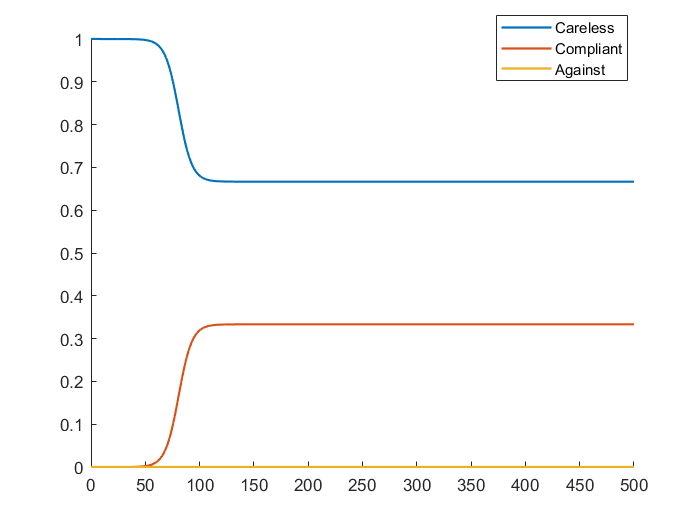
\includegraphics[width=0.7\linewidth]{1_corpo/figure/behavioural_equilibrium/r1greater1_dyn}
	\caption[Behavioural dynamic first case]{The behavioural system dynamic with $R1 > R2$ and $R1 > 1$.}
	\label{fig:r1greater1dyn}
\end{figure}
In this first scenario, as visible in figure \ref{fig:r1greater1dyn}, the Against compartment tend to zero, so the equilibrium point can be calculated as $Ca = \lambda_1/k_1$ and $Co = 1 - \lambda_1/k_1 $. 
The nullcline resulting plot is visible in \ref{fig:r1greater1nullcline}. 
\begin{figure}[h]
	\centering
	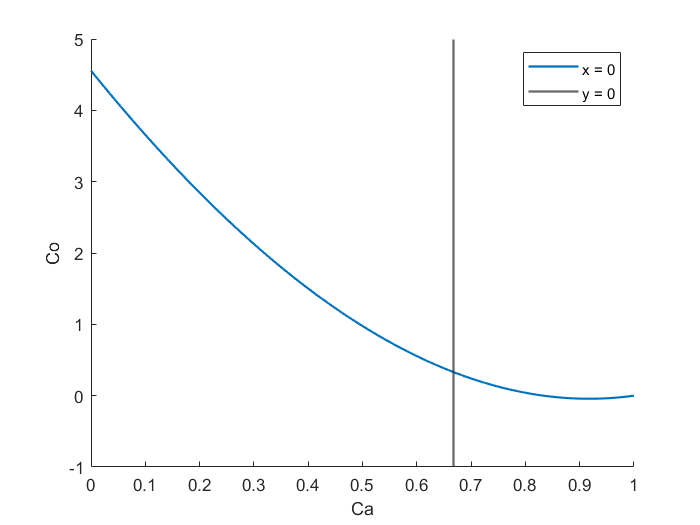
\includegraphics[width=0.7\linewidth]{1_corpo/figure/behavioural_equilibrium/r1greater1_nullcline}
	\caption[Behavioural nullcline first case]{The behavioural system nullcline lines with $R1 > R2$ and $R1 > 1$.}
	\label{fig:r1greater1nullcline}
\end{figure}

The equilibrium found as intersection of the two lines correspond to the one calculated with the numerical equation. With the Routh-Hurwitz criteria the stability of this point is verified. To evaluate if the criteria is satisfied the Jacobian matrix of the system is calculated. Then the equilibrium is used to evaluate the trace and determinant of the system in this value. To see if the equilibrium satisfies Routh-Hurwitz condition it must holds:
\begin{itemize}
	\item trace(J) $< 0$
	\item det(J) $> 0$
\end{itemize}
Both condition holds and the solution is asymptotically stable and does not depends on the initial condition.
%%%%%%%%%%%%%%%%%%

\textbf{II case:} $R_2 >1$ and $R_2> R_1$\\
The plots of the system evolution has an opposite behaviour w.r.t the first case. So here, is the Compliant compartment that tend to zero at equilibrium. 

\begin{figure}[h]
	\centering
	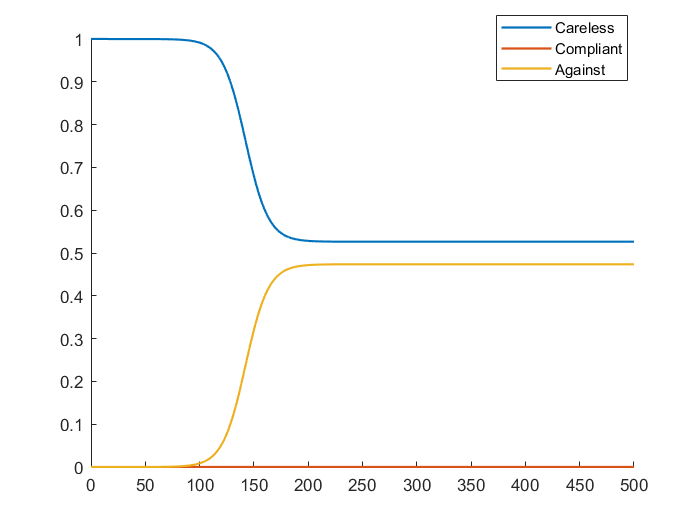
\includegraphics[width=0.7\linewidth]{1_corpo/figure/behavioural_equilibrium/r2greater1_dyn}
	\caption[Behavioural dynamic second case]{The behavioural system dynamic with $R2 > R1$ and $R2 > 1$.}
	\label{fig:r2greater1dyn}
\end{figure}
The equilibrium point can be calculated as $Ca = \lambda_2/k_2$ and $Co = 1 - \lambda_2/k_2$. 
The nullcline resulting plot is visible in \ref{fig:r2greater1nullcline}. 
\begin{figure}[h]
	\centering
	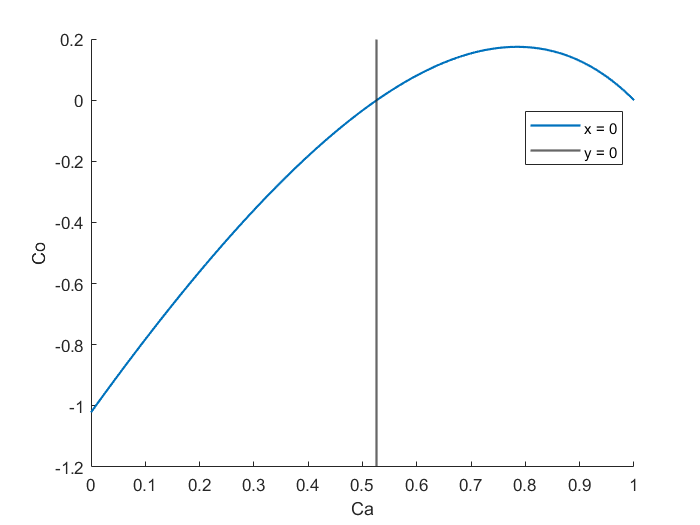
\includegraphics[width=0.7\linewidth]{1_corpo/figure/behavioural_equilibrium/r2greater1_nullcline_1}
	\caption[Behavioural nullcline second case]{The behavioural system nullcline lines with $R2 > R1$ and $R2 > 1$.}
	\label{fig:r2greater1nullcline}
\end{figure}
The equilibrium is asymptotically stable. 
%%%%%%%%%%%%%%%%%%%%%%%%%%%%

\textbf{III case:} $R_1 <1$ and $R_2<1$ \\
If both the "reproduction rates" have a value lower than one, the stable equilibrium is the one in which both Compliant and Against goes to zero. 

\begin{figure}[h]
	\centering
	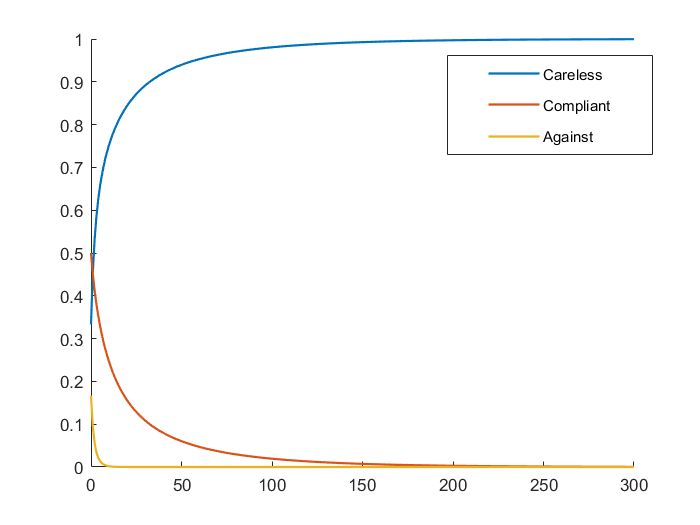
\includegraphics[width=0.7\linewidth]{1_corpo/figure/behavioural_equilibrium/r1r2less1_dyn}
	\caption[Behavioural third second case]{The behavioural system dynamic with $R1 < 1$ and $R2 < 1$.}
	\label{fig:r1r2less1dyn}
\end{figure}
From the nullcline plot \ref{fig:r1r2less1nullcline}, it can be seen that there is not an intersection. The plot of the second nullcline result in a vertical line with a value grater than one. In this condition the only equilibrium is the one for which $Ca = 1$ and both $Ag$ and $Co$ are equal to zero. 
The equilibrium is asymptotically stable. 
\begin{figure}[h]
	\centering
	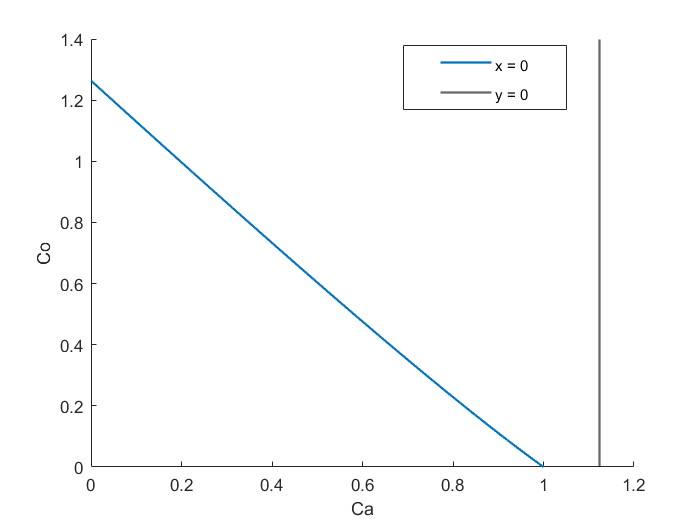
\includegraphics[width=0.7\linewidth]{1_corpo/figure/behavioural_equilibrium/r1r2less1_nullcline}
	\caption[Behavioural nullcline third case]{The behavioural system nullcline lines with $R1 < 1$ and $R2 < 1$.}
	\label{fig:r1r2less1nullcline}
\end{figure}
%%%%%%%%%%%%%%%%%%%%%%%%%%%%

\textbf{IV case:} $R_1 = R_2$ \\
This final situation is the most difficult to analyse. In fact, due to the equal value of the two influence processes, the final equilibrium of the compartments cannot be calculated using only the previous relations, but depends also on the initial condition. 
The Careless compartment can be calculated using the same equation of previous cases, and the same value is found using both $Ca = \lambda_1/k_1$ and $Ca = \lambda_2/k_2$. As it can be seen from the system evolution and nullcline plots \ref{fig:r1r2equaldyn},at the equilibrium the Against and Compliant groups are formed by a subdivision of the $1 - Ca$ part. The initial condition have an influence on how this subdivision is composed. Using the Routh-Hurwitz criterium nothing can be said on this equilibrium because the determinant of the Jacobian have a null value.
\begin{figure}[h]
	\centering
	\subfloat[][\emph{System  evolution.}]
	{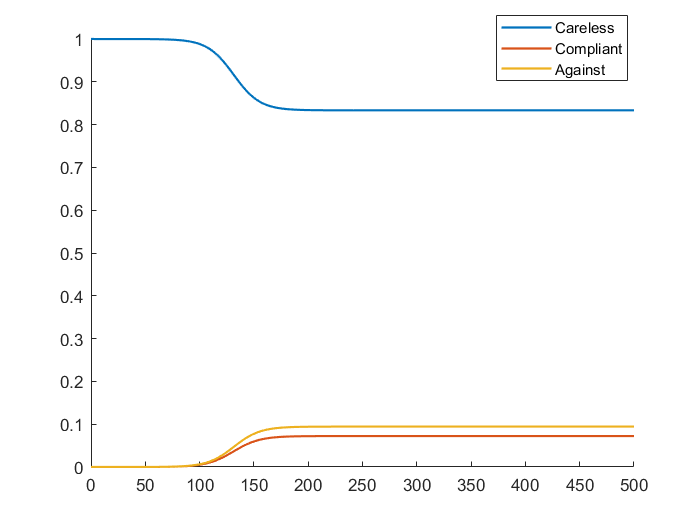
\includegraphics[width=0.47\linewidth]{1_corpo/figure/behavioural_equilibrium/r1equalr2_dyn}} \quad
	\subfloat[][\emph{Nullclines plots.}]
	{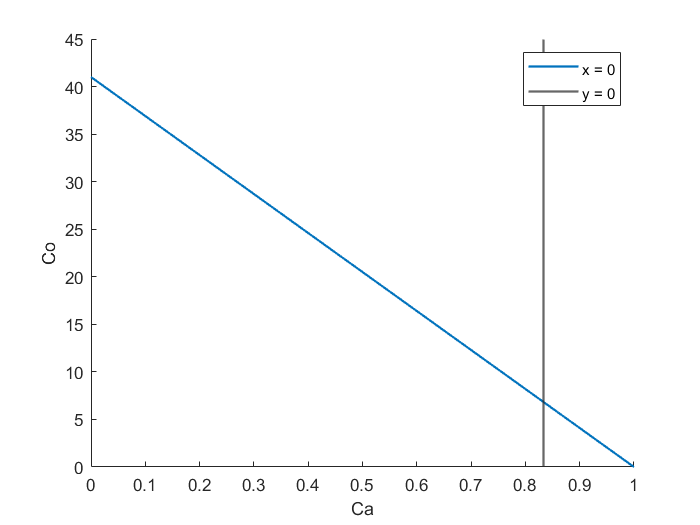
\includegraphics[width=0.47\linewidth]{1_corpo/figure/behavioural_equilibrium/r1equalr2_nullcline}} \\
	\caption[Behavioural model fourth case]{Behavioural system dynamics and nullcline in the case of   $R_1 = R_2$.}
	\label{fig:r1r2equaldyn}
\end{figure}

\subsubsection{Behavioural model experiment}
To better comprehend all the possible scenarios that can emerge with the behavioural model a simulation is performed. Four vectors are defined, one for each parameter of the model. A different simulation for each combination of the coefficient is then roll out. In this case the value of the parameters is kept constant during each simulation.
The range of variation of each parameter is the following:
\begin{itemize}
	\item $k_1$ between $0.1$ and $0.99$
	\item $k_2$ between $0.1$ and $0.99$
	\item $\lambda_1$ between $1/5$ and $1/30$ $d^{-1}$
	\item $k_1$ between $1/5$ and $1/30$ $d^{-1}$
\end{itemize}
We observe the evolution of the dynamics of all the states, and to present a summary of the effects we collect for each simulation data such as the final value of the compartment, the max peak value and the corresponding time in which the peak occur. 
Also here, for the sensitivity plots realization, the reproduction rates deriving from the combination of coefficients, equation \ref{eq:behave_rate}, are used. 

The first plots \ref{fig:subfig_sensitivity_behavioural} are heat maps about the final value reached by various compartments, varying $R_1$ and $R_2$.

\begin{figure}[h]
	\centering
	\subfloat[][\emph{Final Compliant compartment}]
	{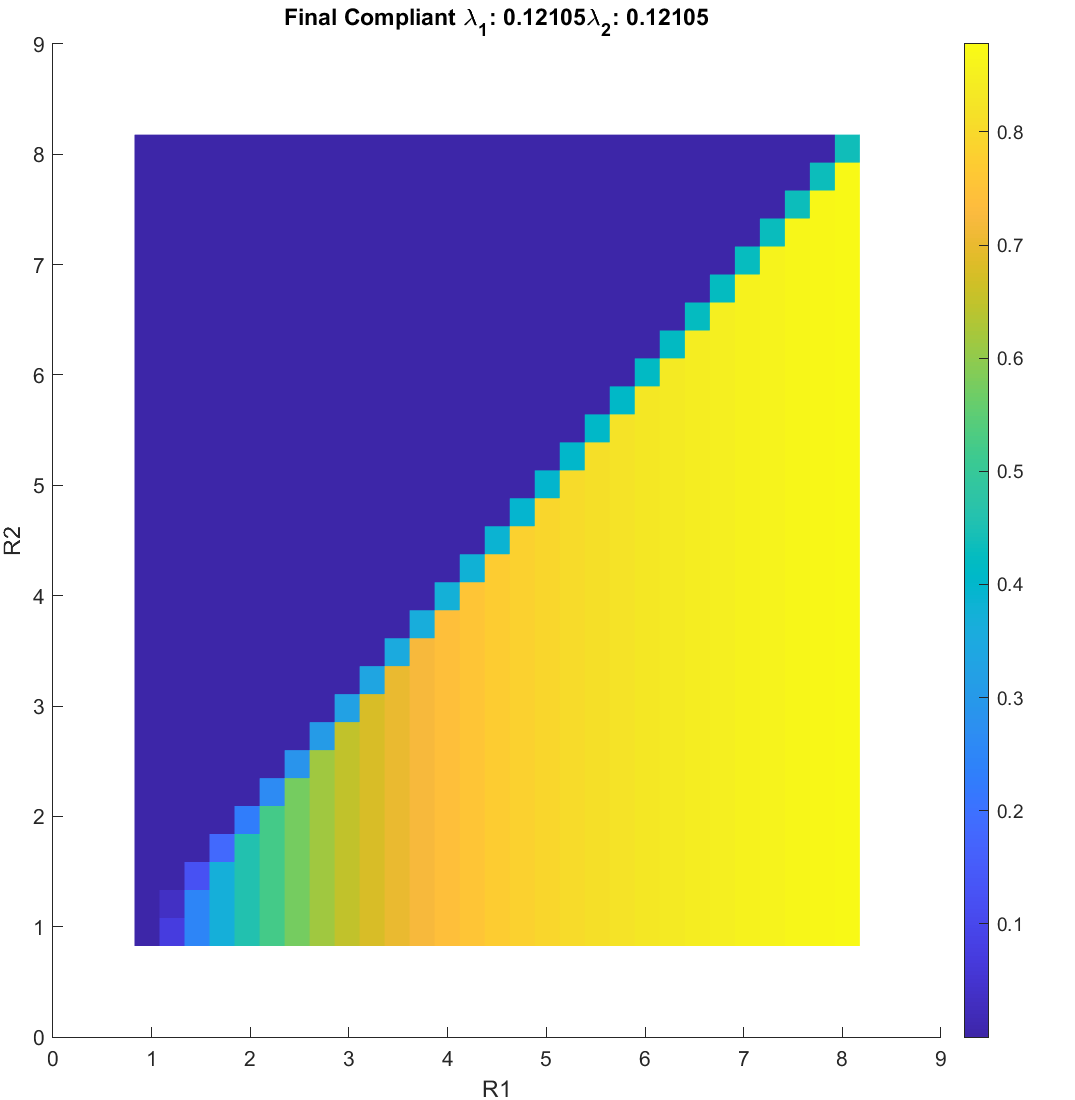
\includegraphics[width=.47\textwidth]{1_corpo/figure/behavioural_equilibrium/final_compliant_sensitivity}} \quad
	\subfloat[][\emph{Final Against compartment}]
	{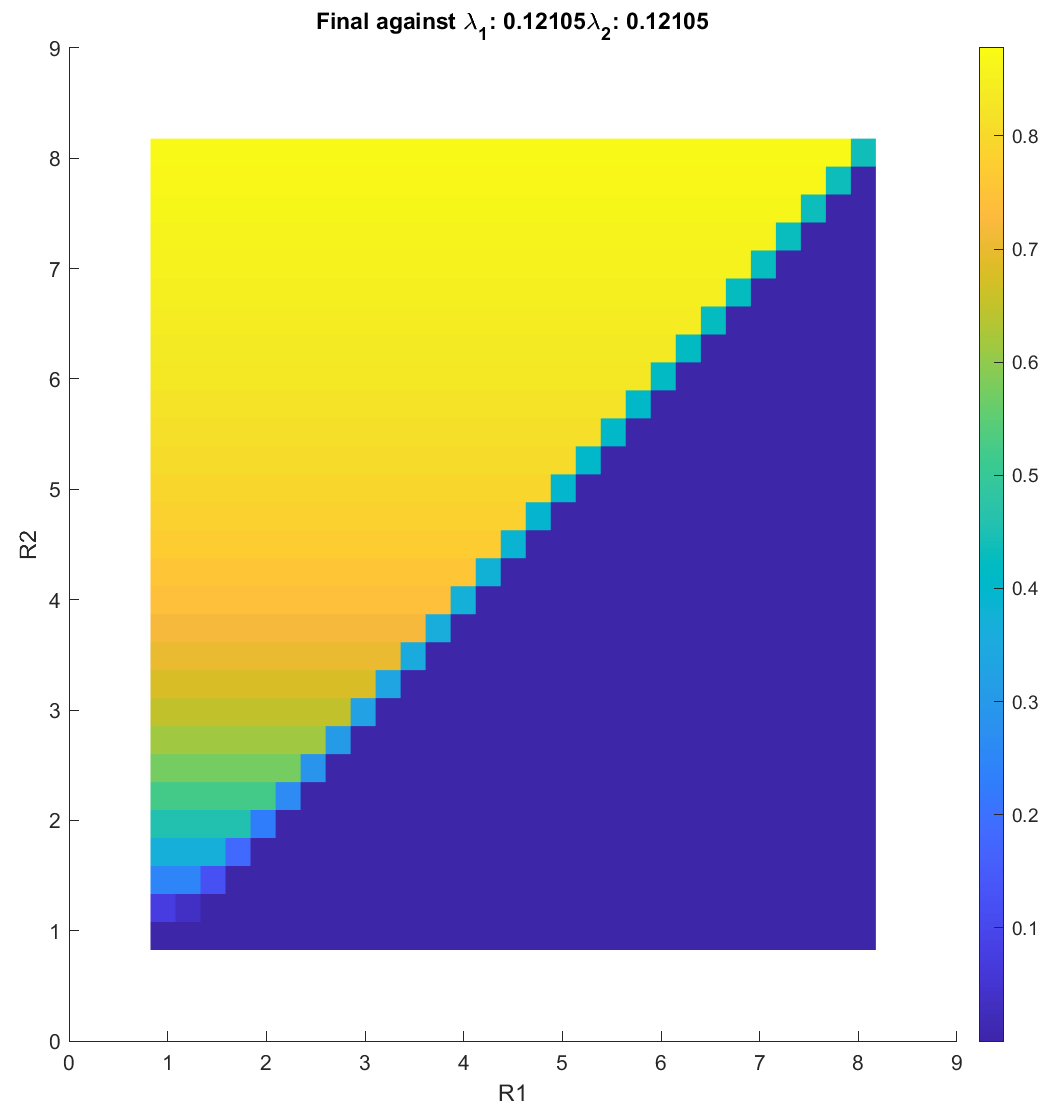
\includegraphics[width=.47\textwidth]{1_corpo/figure/behavioural_equilibrium/final_against_sensitivity}} \\
	\subfloat[][\emph{Final Careless compartment}]
	{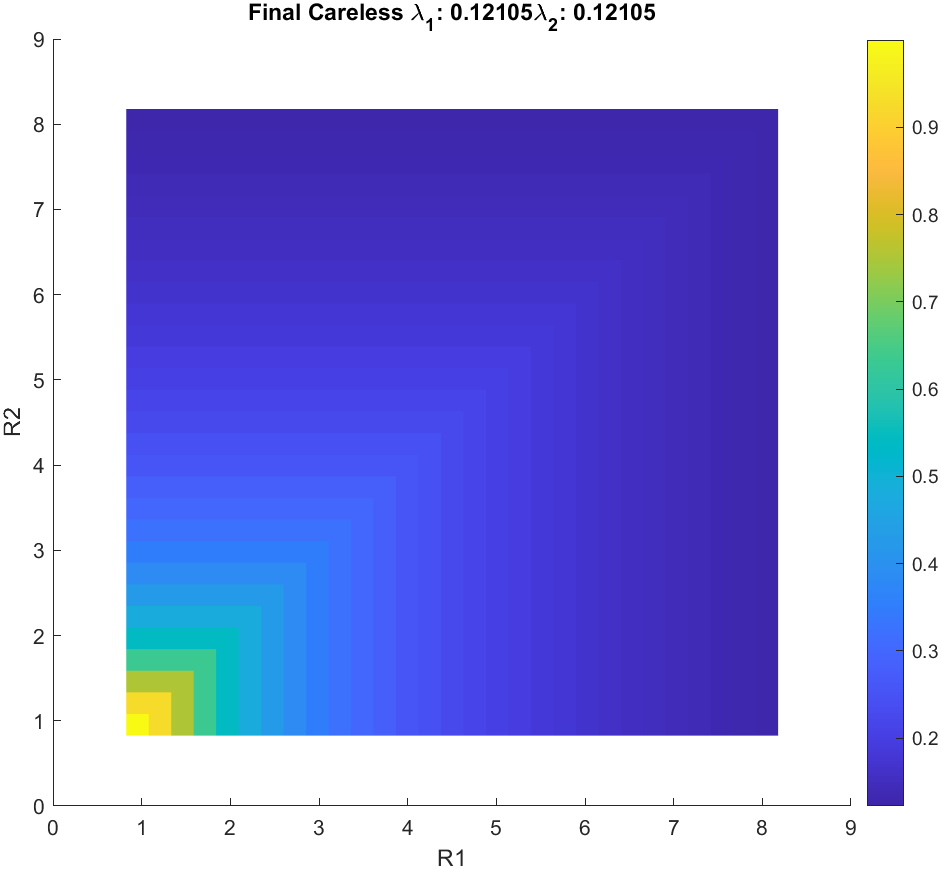
\includegraphics[width=.47\textwidth]{1_corpo/figure/behavioural_equilibrium/final_careless_sensitivity}}
	\caption[Final Behavioural compartments]{The final value reached at equilibrium by every compartment in the behavioural model.}
	\label{fig:subfig_sensitivity_behavioural}
\end{figure}

In these pictures is clearly visible the threshold effect observed in the stability analysis performed earlier. While one of the reproduction ratios becomes larger than the other, the system equilibrium is composed by the dominant group and a portion of Careless individuals.The greater is the ratio, the  smaller is the size at equilibrium of the Careless. 

Another figure in which this threshold effect can be observed is \ref{fig:subfig_sensitivity_behavioural_r1}.

\begin{figure}[h]
	\centering
	\subfloat[][\emph{Final Compliant compartment}]
	{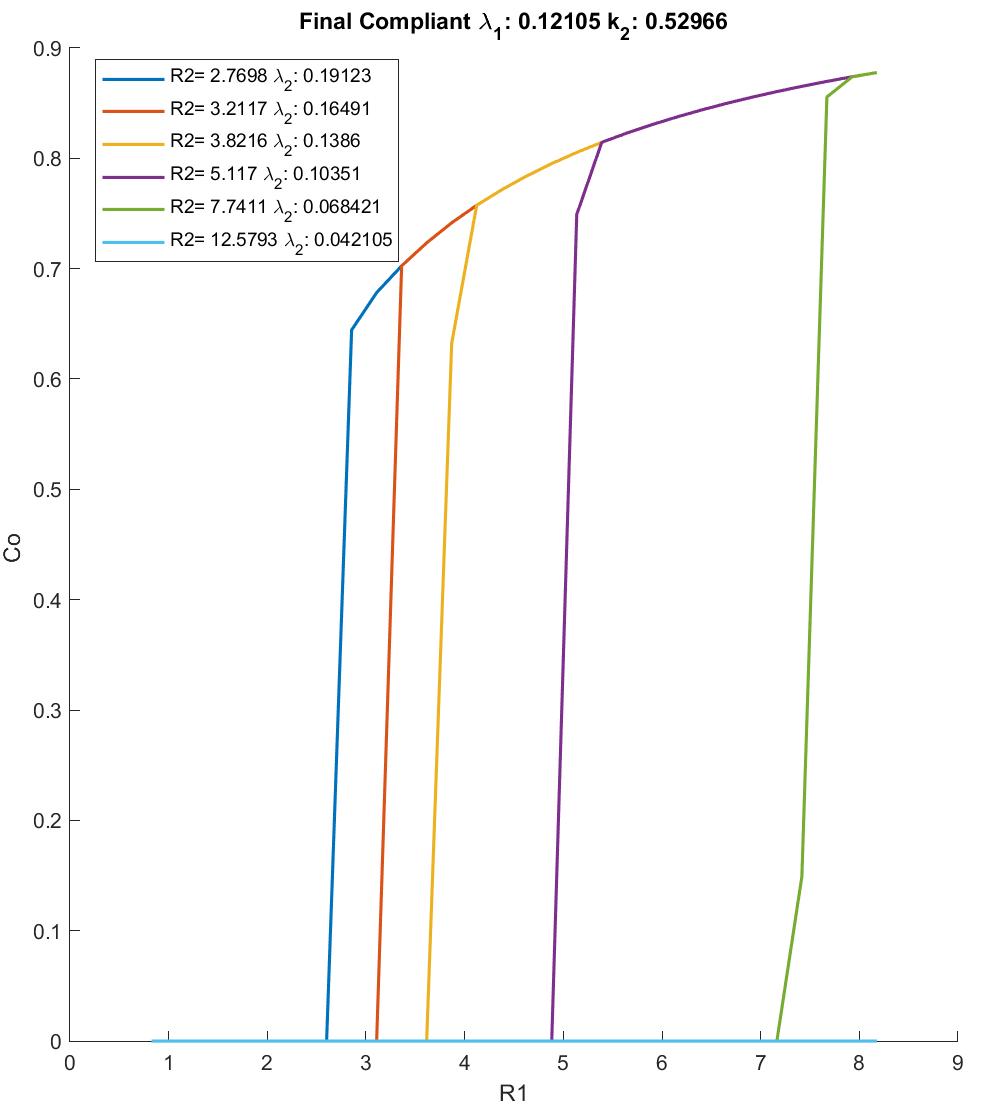
\includegraphics[height=.45\textwidth]{1_corpo/figure/behavioural_equilibrium/final_compliant_r1}} \quad
	\subfloat[][\emph{Final Against compartment}]
	{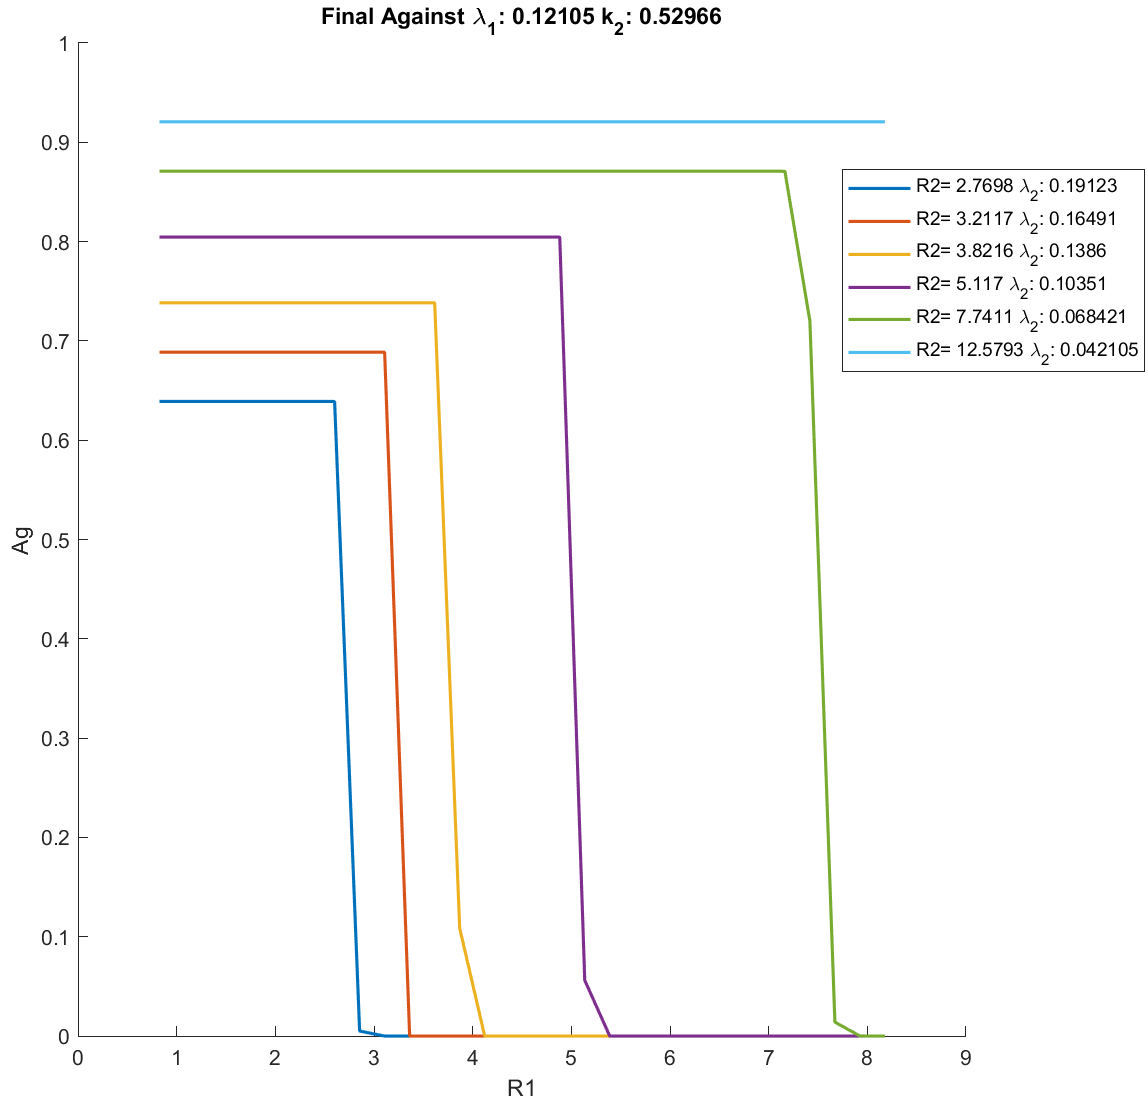
\includegraphics[height=.45\textwidth]{1_corpo/figure/behavioural_equilibrium/final_against_r1}} \\
	\subfloat[][\emph{Final Careless compartment}]
	{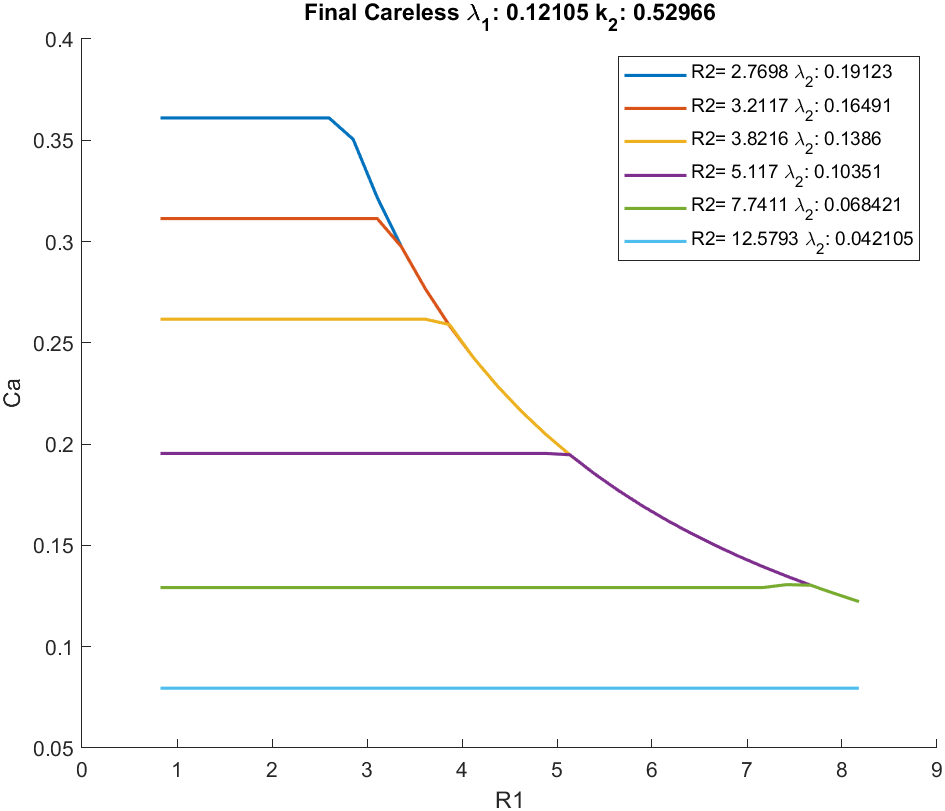
\includegraphics[height=.45\textwidth]{1_corpo/figure/behavioural_equilibrium/final_careless_r1}}
	\caption[Final Behavioural compartments varying $R_1$]{The final value reached at equilibrium by every compartment in the behavioural model varying the $R_1$ coefficient w.r.t different $R_2$ values.}
	\label{fig:subfig_sensitivity_behavioural_r1}
\end{figure}
The plots show how, for a fixed values of $\lambda_1$ and $k_2$, change the size at equilibrium of the system, varying the $k_1$ coefficient. To highlight the threshold effect due to the comparison of reproduction rates, on the x-axis is plotted the $R_1$  coefficient, that can be calculated knowing the value of  $\lambda_1$ and $k_1$. For the same reason, different $R_2$ situations are represented. 

The threshold effect is clearly visible also here. Looking at the Compliant and Against final values it can also be seen that after the $R_1$ reproductive coefficient is became dominant, the  increase is the final size observed in the Compliant plot is due to the decrease in the Careless compartment. 

Provo a scrivere, ma si va tutto molto bene
L'inglese, come disse Daniele è da sistemare, però sono su una buona strada...